%----------------------------------------------------------------------------------------------
\chapter{LITERATURE REVIEW OF GEOMETRIC MODELING}
\label{Literature Review}
\lhead{Chapter 2. \emph{Literature Review}}

%----------------------------------------------------------------------------------------
%      INTRODUCTORY PARAGRAPHS
%----------------------------------------------------------------------------------------

\hspace{30} With the advent of computers which could perform millions of floating
point operations in unit time and which are still growing faster, researchers who
believed computers could aid the processes of mechanical design and
manufacturing were faced with a critical issue – how to represent physical
reality using computer software. They sought the best data structures to
represent this reality and the most appropriate algorithms to manipulate these representations.

\hspace{30} BRL-­CAD supports a wide variety of geometric representations including an 
extensive set of traditional implicit primitive shapes as well as explicit primitives
made from collections of uniform B­spline surfaces, non­uniform rational B­spline (NURBS)
surfaces, n­on-manifold   geometry   (NMG)   and purely faceted polygonal mesh geometry.
Consequently, in this chapter, we review the existing work done by scholars in the 
field of geometric modeling which have been applied to the development of BRL-­CAD. 
First of all, it introduces the issue of representation and the notion of representation
 schemes. Then, it summarizes developments in wireframe modeling, surface modeling, solid
modeling and non­-manifold modeling (aka non­manifold geometry or nmg for short) with a keen
 eye on the algorithms underlying them.

\hspace{30} As we progress in our literature review from older forms of geometric
modeling to newer ones, we will discover that representation schemes were
closely linked to algorithmic efficiency and that it has always been normal to
expect designers to switch to newer ones in response to the improvements in
algorithmic performance.Despite these enhancements in algorithmic efficiency
within the designer community, we cannot say with complete certainty whether
traditional representation schemes have been relegated to the background. We
can only conclude that old and new representation paradigms co­exist and that
research led to representation schemes which supplemented the repertoire of
geometric modeling.  

%-----------------------------------------------------------------------------------------

%----------------------------------------------------------------------------------------
%	SECTION 1
%----------------------------------------------------------------------------------------

\section{Representation Schemes}
\theoremstyle{definition} \newtheorem{Def1}{Definition}[section]
\theoremstyle{remark} \newtheorem{Def2}{Remark}[section]
\begin{Def1}
A representation $\textbf{\mathfrak{R}}$ of a solid or representation for short is a subset of
three­-dimensional Euclidean space denoted $\mathbb{E}^3$ which models a physical solid.
\end{Def1} According to \cite{5}, Requicha and Tilove stated that point set topology provided a
formal language for describing the geometric properties of solids and they also  
threw more light on the mathematical characteristics of solids such as a solid's
interior, boundary, complement, closure, boundedness and regularity.
Requicha \cite{4} insisted that to be computationally useful, a representation should  
formally capture the following properties ;

\begin{itemize}
\item \textit{\textbf{Rigidity:}} Representations should have an invariant configuration
irrespective of their location and orientation.
\item \textit{\textbf{Homogeneity:}} A representation should have an interior.
\item \textit{\textbf{Finiteness:}} A representation must occupy a finite amount of space.
\item \textit{\textbf{Boundary   determinism:}} A representation must unambiguously determine
the interior of that solid.
\item \textit{\textbf{Closure}}: Representations of solids which are manipulated by rigid
motions and regularized boolean operations should produce representations of solids too.
\end{itemize}
These formal characteristics leave representations no choice than to be
bounded, closed, regularized and semi­analytic, hence their coinage \textit{\textbf{r-­sets}}
according to \cite{5}. 
\begin{Def2}
An \textit{\textbf{r - ­set}} is simply a regular and bounded set in $\mathbb{E}^3$.
\end{Def2}
\hspace{30} A representation scheme is simply a relation between physical solids and their representations which can be characterized by the following properties;
\begin{itemize}
\item \textit{\textbf{Domain}}: A representation scheme must represent quite a number of useful geometric solids. 
\item \textit{\textbf{Unambiguity}}: A representation scheme should produce representations which intuitively capture the properties of the physical solid so that it can be easily distinguished from other representations.
\item \textit{\textbf{Uniqueness}}: A representation scheme should uniquely represent a solid object within a software's database.  
\item \textit{\textbf{Validity}}: Representation schemes should yield representations of solids which do not exist or are valid.  
\item \textit{\textbf{Closure}}: A Representation scheme which transforms (reflects, scales, rotates) a representation should yield other representations too.
\item \textit{\textbf{Compactness}}: Representation schemes should yield representations which save space and allow efficient algorithms to   determine desirable physical characteristics.
\end{itemize}
%--------------------------------------------------------------------------------------------------
%	WIREFRAME MODELING
%-----------------------------------------------------------------------------------------------------
\section{Wireframe Modeling}

For rectilinear objects whose edges are straight lines and whose faces are planar, the ordered pair of vertices
 $\textbf{\mathfrak{V}} \in \mathbb{E}^3$ and edges $\textbf{\mathfrak{E}} \in \mathbb{E}^3$ denoted by $(\textbf{\mathfrak{V}} , \textbf{\mathfrak{E}})$ is the object's wireframe.  
In a practical sense, it is the skeleton of an object wherein joints are vertices
and bones are edges. In \cite{6}, a six ­step algorithm to generate an object's
wireframe was developed wherein an object's wireframe was represented by a vertex table and an edge table. 
Although the work in \cite{6} had drawbacks such as not checking the validity of input data, wireframe modeling has always provided designers with a chance to experiment with the final result of their models through sketching and it is frequently used to preview complex models. However, the use of only edge information left wireframe models ambiguous
on both rectilinear and topological polyhedra. Figure 2.1 below shows the wireframe of a sphere in greyscale.

%--------------------------------------------------------------------------------------------

\begin{figure}[htbp]
\centering
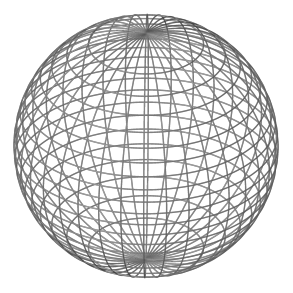
\includegraphics[trim=0.1cm 0.3cm 0.5cm 0.5cm, clip=true, totalheight=0.5\textheight]{Figures/Sphere.png}
\caption[A wireframe of a sphere]{A wireframe of a sphere}
\label{Sphere}
\end{figure}

%--------------------------------------------------------------------------------------------

%----------------------------------------------------------------------------------------
%	SURFACE MODELING
%----------------------------------------------------------------------------------------

\section{Surface Modeling}

After breakthroughs in wireframe modeling, research efforts in geometric modeling were directed 
towards extending the geometric coverage of CAD packages by incorporating complex free­form surfaces
 and curves. In this section, we emphasize on algebraic surfaces and curves, the basis for Bezier 
surfaces and NURBS used within BRL­-CAD.

%--------------------------------------------------------------------------------------------

\begin{figure}[htbp]
\centering
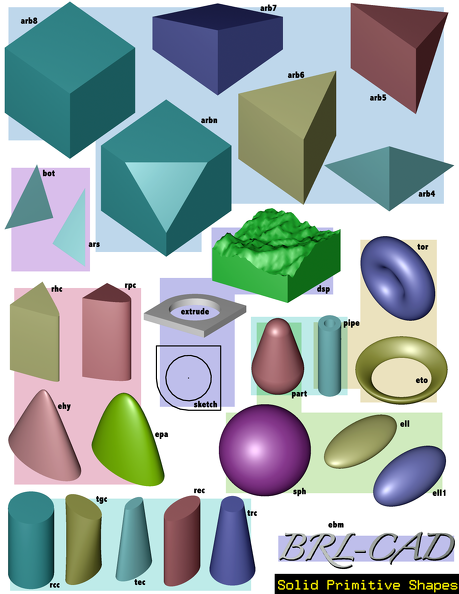
\includegraphics[trim=0.1cm 0.3cm 0.5cm 0.5cm, clip=true, totalheight=0.6\textheight]{Figures/Primitives.png}
\caption[BRL­-CAD Solid Primitive Shapes]{BRL-­CAD Solid Primitive Shapes}
\label{Primitives}
\end{figure}

%--------------------------------------------------------------------------------------------

Figure 2.2 above shows a collection of some primitives used within the BRL-­CAD package before the heart-­shaped primitive   was developed – several of which are implicitly and/or parameterically represented by algebraic equations. On the BRL-­CAD's ideas page \cite{7}, there is a list of primitives which have not yet been implemented such as the Steiner surface, the ring 
cyclide surface, the quartoid, Wallis' conical edge solid, etc.  

%----------------------------------------------------------------------------------------------------
%	Implicit Representations
%----------------------------------------------------------------------------------------------------

\subsection{Implicit Representation}

An algebraic surface in $\mathbb{E}^3$ is expressed as the set of points satisfying an irreducible polynomial equation
\begin{equation*}
\textbf{g(x,y,z) = 0}
\end{equation*} in the unknowns x,y and z.
\theoremstyle{remark} \newtheorem{Def3}{Definition}[section]
\begin{Def3}
A polynomial \textit{\textbf{f(x,y,z)}} over a field $\textbf{\mathbb{F}}$ is said to be irreducible over $\textbf{\mathbb{F}}$ if the degree of \textit{\textbf{f(x,y,z)}} is positive and its only factors are \textit{c} and \textit{cf(x,y,z)} where \textit{c} is a non­zero constant in $\textbf{\mathbb{F}}$.
\end{Def3}
The requirement of irreducibility is so that a surface represented by an equation
should not be decomposed into two separate surfaces, each of which can be
described by an implicit equation.

%------------------------------------------------------------------------------------------------------

%------------------------------------------------------------------------------------------------------
%	Parametric Representations
%------------------------------------------------------------------------------------------------------

\subsection{Parametric Representation}

Some algebraic surfaces possess a parametric representation which  
consists of a system of equations similar to the ones listed in (1) below;  

\begin{IEEEeqnarray*}
\centering
x = h_1(u,v)  \\
y = h_2(u,v) ­­­­­­­­­­­­­­­­­­­­­­­­­­­­­\IEEEyesnumber \\
z = h_3(u,v) \\
\end{IEEEeqnarray*} where $h_i$ are rational functions and, u and v are restricted to particular closed intervals in $\mathbb{R}$.

As an example, the unit sphere given implicitly by $x^2 + y^2 + z^2 – 1 = 0$ can be parameterized by equation (2) viz;

\begin{IEEEeqnarray*}
\centering
x = (1 – s^2 - t^2)/(1 + s^2 + t^2) \\  
y = 2s / (1 + s^2 + t^2) \IEEEyesnumber \\
z = 2t / (1 + s^2 + t^2) \\
\end{IEEEeqnarray*}

Also, some algebraic curves possess parametric forms. A parameterization of the unit circle is given by the system of  equations in (3) below;

\begin{IEEEeqnarray*}
\centering
x = (1 – t^2)/ (1 + t^2)­ \\
y = 2t / (1 + t^2) \IEEEyesnumber \\
\end{IEEEeqnarray*}

When the parametric representation is employed, it is easier to generate points on an algebraic surface or curve as compared to the implicit representation. Also, parametric equations are useful for interactive design
since changes in their polynomial coefficients alter the surface's shape in an intuitive manner.

Lots of geometric operations could become faster if both
aforementioned representations are made available within CAD packages.
Thus, the problem of how to convert from one representation to the other is of
great importance.

%------------------------------------------------------------------------------------------------------

%------------------------------------------------------------------------------------------------------
%		IMPLICITISATION
%------------------------------------------------------------------------------------------------------

\subsection{Implicitization}

Implicitization is the process of converting a parametric representation into an implicit representation.
Sederberg \cite{7} demonstrated in his thesis that, in principle, it is always
possible to convert a parametric surface or curve into implicit form using
classical elimination theory developed in the early $20^{th}$ century. In fact,
Sylvester resultants require evaluating a determinant whose entries are
coefficients of powers of the variable to be eliminated in several phases.

\hspace{20}Although Sederberg’s work stimulated lots of research interests in resultant­-based methods, 
this sense of enjoyment within the research community was short­lived due to the following factors;
\begin{itemize}  
\item ✦ Unfaithfulness: Polynomials derived using resultant-­based methods give
birth to phantom solutions.
\item ✦ Ineffectiveness: Using floating ­point arithmetic, resultant­-based methods  
become inaccurate.
\item ✦ Inefficiency: Evaluating resultants entail huge amounts of computation
and is expensive.
\end{itemize}
Another method of Implicitization is the Gr\"\o bner basis technique introduced by
Buchberger \cite{8} where it was learned that expressing a polynomial as a linear
combination of a Gr\"\o bner basis facilitates finding the solution of the nonlinear
system of equations as  much as an $\textbf{\mathbb{LU}}$ - ­decomposition brings a system of
linear equations to heel. 
\theoremstyle{remark} \newtheorem{Def4}{Definition}[section]
\begin{Def4}
A polynomial basis is a set of polynomials which
can be used to express any polynomial and can be viewed as a vector space
over the field of coefficients $\mathbb{F}$.
\end{Def4} 
\hspace{20}In \cite{9}, Lazard constructed a Gr\"\o bner basis with  
respect to a term ordering known as the elimination order. In \cite{10}, Hoffmann
improved upon a basis conversion algorithm developed in \cite{11} by first
constructing a Gr\"\o bner basis with respect to a term ordering different from the  
elimination order and finally built the final polynomial in which all variables have
been eliminated term ­by ­term. This algorithm was known to be the fastest
elimination technique for geometry applications that was implemented before
the 1990s.

\hspace{20}Although Gr\"\o bner basis methods are more efficient and effective than
resultant-­based ones, implicitization is fairly expensive and limited in practice.  

%------------------------------------------------------------------------------------------------------


%------------------------------------------------------------------------------------------------------
%		PARAMETERIZATION
%------------------------------------------------------------------------------------------------------

\subsection{Parameterization}

Parameterization is the process of converting an implicit representation of 
an object into its parametric equivalent, if it exists. Parameterization is not
always possible since not all implicit surfaces can be expressed as rational
parameterizations. Noether's theorem states that a plane algebraic curve
possesses a rational parameterization if and only if it has genus zero. \cite{13} used
a numerically stable Jacobi rotation adapted from \cite{12} to parameterize several
conics and parametric surfaces. Table 2.1 below shows a list of
parameterizations of some popular conics – circle, ellipse, hyperbola and
parabola.
\begin{table}[thbp]
\caption[Implicit and parametric equations of some BRL-­CAD primitives]{Implicit and parametric equations of some BRL­-CAD primitives}
\centering
\begin{tabular}{| l | c | c |}
  \hline
   & Implicit Form & Parametric Form &  \\
  \hline
  Circle & $x^2 + y^2 - r^2 = 0$ &    $x =  \frac{r(1 – t^2)}{(1 + t^2)}$ , $y = \frac{2rt}{(1 + t^2)}$ \\
  \hline
  Ellipse & $\frac{x^2}{a^2} + \frac{y^2}{b^2} - 1 = 0$ &     $x = \frac{a(1 – t^2)}{(1 + t^2)}$, $y = \frac{2bt}{(1 + t^2)}$ \\
  \hline
  Hyperbola & $\frac{x^2}{a^2} - \frac{y^2}{b^2} - 1 = 0$ &     $x = \frac{a(1 + t^2)}{(1 - t^2)}$, $y = \frac{2bt}{(1 - t^2)}$ \\
  \hline
  Parabola & $y^2 - 2px = 0$ &     $ x = \frac{t^2}{2p}$, $ y = t$ \\
  \hline
\end{tabular}
\label{Implicit and Parametric equations}
\end{table}

\clearpage
%------------------------------------------------------------------------------------------------------

%------------------------------------------------------------------------------------------------------
%	SOLID MODELING
%------------------------------------------------------------------------------------------------------

\section{Solid Modeling}

\hspace{30} A solid can be represented explicitly by its boundary, its volume, or
implicitly by specifying operations on volumetric properties that construct it.
BRL-­CAD focuses on solid modeling by emphasizing physical accuracy and
fully describing $\mathbb{E}^3$.

There are 3 main well­ established paradigms for representing solids used
within BRL-­CAD based on their boundaries, volumes or constructing from
primitives using regularized boolean operations, a boolean set theoretic
operations applied to the context of r­sets which were developed in \cite{4}.

In this section, we review the literature that has grown around classical
representation paradigms such as \textit{Boundary   Representations}, \textit{Constructive  
Solid Geometry} and \textit{Spatial subdivision.}

\subsection{Boundary Representations (B-REPS)}

\hspace{30} Just as Rome was not built in a day, the transition from surface modeling
representation schemes   to   solid   modeling   representation   schemes   was   a  
gradual   process   which   started   off   with   boundary   representations.   The   boundary  
representations   popularly   known   as   as   B­REPS   describe   a   solid   as   a   set   of  
surfaces which separate an object's interior from its exterior. 

\hspace{30} With   B­REPS,   the   boundary   of   a   solid   consists   of   vertices,   edges   and  
faces.   For   each   vertex,   edge   and   face,   the   geometric   section   of   the  
representation   holds   the   shape   and   location   of   the   object   in   space   possibly  
using   an   equation   while   the   topological   section   of   the   representation   holds   the  
adjacency   relationships   between   the   vertices,   edges   and   faces   as   well   as   their  
orientation.   There   are   nine   (9)   ordered   adjacency   relationships   between   the  
three   (3)   aforementioned   topological   entities.   In   order   to   build   a   complete  
representation,   it   is   normal   for   one   to   allow   the   retrieval   of   any   topological   entity  
and   any   of   the   nine   (9)   ordered   adjacency   relationships. Kevin Weiler \cite{14}  
showed   that   only   three   (3)   ordered   adjacency   relationships   are   sufficient   to  
obtain   the   others.   From   his   work   ,a   space/time   trade­off   arose:   Maintaining   all   9  
adjacency   relationships   required   more   space   but   little   time   for   retrieval   while  
maintaining   only   sufficient   adjacency   relationships   required   little   space   but  
more   time   for   retrieval.   A   more   indepth   comparison   of   the   space/time  
trade­offs of different boundary representations was conducted by Woo \cite{15}.  

\hspace{30} For   solids   with   a   manifold   surface,   several   boundary   representations  
exist,   the   earliest   of   which   was   Baumgart's   \textbf{winged ­edge}   data   structure   \cite{16}.  
Here,   an   edge   node   holds   information   about   the   edge   orientation,   face  
adjacencies   and   the   clockwise/counterclockwise   successor   and   predecessor  
edges   about   adjacent   faces.   This   work   was   based   on   the   assumption   that  
faces   are   simply   connected.   The   winged ­edge   data   structure   has   to   be  
modified   to   accommodate   solids   with   multiply   connected   faces   which   contain  
holes   (genus).   In   \cite{17},   Braid   et   al   modified   the   winged ­edge   data   structure   by  
introducing   a   fourth   topological   entity   called   a   loop   into   a   proposed   data  
structure   where   each   face   consists   of   one   or   more   edge   loops   surrounding  
each   hole   in   that   face.   In   the   same   vein,   Yamaguchi   and   Tokieda   \cite{18}   modified  
the   winged ­edge   data   structure   by   introducing   yet   another   topological   entity  
called   the   bridge   edge   (or   auxillary   edge   which   is   simply   a   double   edge 
connecting two (2) edge cycles of a given face.  

\hspace{30} The   reader   is   invited   to   explore   other   existing   boundary   representations  
such   as   the   half­edge   data   structure   by   Mantyla   \cite{19},   Hanharan's   \textbf{face ­edge}  
representation   \cite{20}   and   Ansaldi   \textit {et al}'s   hierarchical   \textbf{face   adjacency}   hypergraph  
\cite{21}.   In   order   to   accomodate   solids   with   internal   cavities   and   permit   single  
volumes   to   contain   multiple   faces,   a   new   topological   entity   called   the   shell   was  
introduced   in   \cite{21}.   As   regards   conversion,   Shapiro   and   Vossler   \cite{22}   developed  
an   algorithm   which   converts   a   boundary   representation   to   an   equivalent   CSG  
representation in two-­dimensional space.

\hspace{30} The   Euler - ­Poincare   characterization   has   been   used   as   a   necessary  
condition   for   the   validity   of   a   solid   using   its   topological   information   viz   edges  
(E),   vertices   (V),   faces   (F),   loops   (L),   Holes   (G)   and   shells   (S).   It   is   given   by   the  
equation (5) below.
\begin{equation*}
\centering
 V – E + F -­ ( L – F ) - 2(S – G ) = 0 ­­­­­­­­­­­­­­ \tag{5}
\end{equation*}
Mantyla   showed   that   any   topologically   valid   polyhedron   can   be   constructed  
from   an   initial   polyhedron   by   a   finite   sequence   of   Euler   operations   viz   \textit{\textbf{make}}  
and \textit{\textbf{kill}}.

\hspace{30} Some   representation   schemes   are   hybrids   such   as   the   B-­rep   index   which  
is   a   mixture   of   the   boundary   representation   and   cell   decomposition   schemes.  
BRL-­CAD   is   one   of   the   few   solid   modeling   systems   which   supports   the  
BREP and NURBS   representation   format.  The   image   shown   in   Figure   2.3   below   is   the   classic   computer   graphics   Utah  teapot model prepared for 3D printing and rendered via BRL-­CAD ray tracing.\\

\begin{figure}[htbp]
\centering
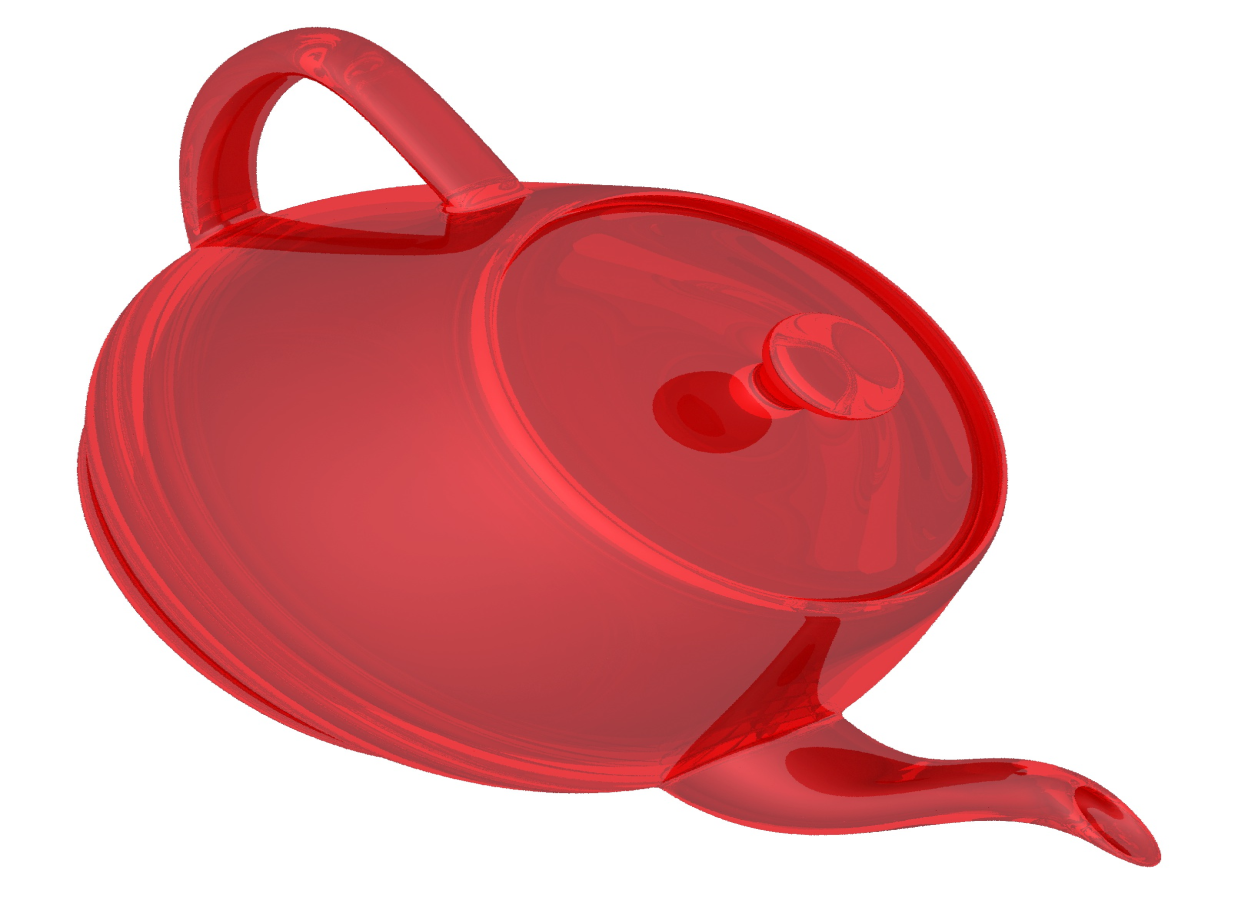
\includegraphics[trim=0.0cm 0.3cm 0.3cm 0.3cm, clip=true, totalheight=0.5\textheight]{Pictures/Teapot.png}
\caption[The Utah Tea Pot model]{The Utah Tea Pot model}
\label{Teapot}
\end{figure}
 
\subsection{Constructive Solid Geometry (CSG)}

\hspace{30} During   the   $18^{th}$   century,   George   Boole's   work   on   the   algebra   of   logic   gave  
birth   to   an   algebra   attributed   to   his   name   called   Boolean   algebra   which  
possessed   its   own   set   theoretic   concepts   and   operations   like   union,  
intersections,   difference   and   complement.   Although   these   operations  
seemed   to   be   obvious   candidates   for   combining   solids,   the   conventional  
aforementioned   boolean   operations   had   been   discovered   to   be   inadequate   to  
manipulate   solids   in   $\mathbb{E}^3$ because   the   regularity  
and   compactness   of   solids   became   compromised.   In   fact,   the   complement  
operator   destroys   the   compactness   of   solids   because   the   complement   of   an  
r­set   is   unbounded.   Thus,   the   need   to   develop   new   kinds   of   set   theoretic  
operations   which   work   well   within   the   realm   of   solid   modeling   was   of   paramount  
importance.   In   \cite{23},   Requicha   developed   a   new   set   of   operations   peculiar   to  
r­sets   called   \textit{regularized   union},   \textit{regularized   intersections}   and   \textit{regularized  
difference}.

\hspace{30} His   work   even   went   forward   to   show   that   the   r­sets   and   the   regularized  
boolean   operations   formed   not   just   a   boolean   algebra   but   also   a   ring.   Besides  
these   regularized   boolean   operations   on   solids,   there   also   existed   other   valid  
operations   on   r­sets   which   are   linear   transformations   viz   reflection,   scaling,  
rotation,   shearing,   etc.   The   image   in   Figure   2.4   below   illustrates   how   the  
regularized boolean operations result to new shapes.

\begin{figure}[htbp]
\centering
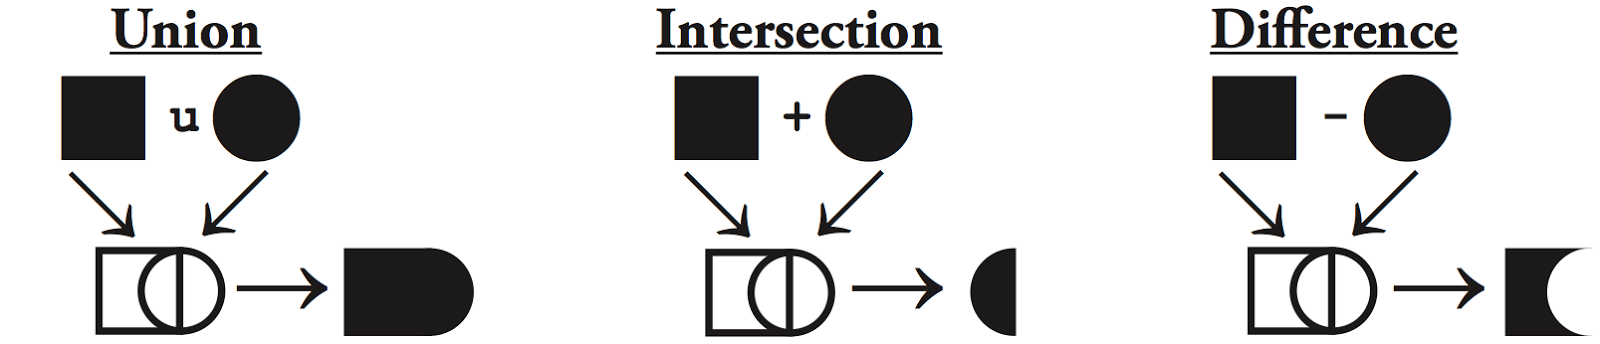
\includegraphics[trim=0.0cm 0.5cm 0.1cm 0.1cm, clip=true, totalheight=0.12\textheight]{Pictures/Boolean.png}
\caption[CSG Boolean operations]{CSG Boolean operations}
\label{Boolean}
\end{figure}

\hspace{30} One of the most widely used representation schemes of our time
combines the volumes occupied by overlapping r­sets using regularized
boolean operations. This representation scheme is called Constructive Solid
Geometry (CSG) and its signature is the CSG tree – a binary tree data
structure whose leaves are primitives and whose internal nodes are either
regularized boolean operations or linear transformations. By a primitive, we
simply mean a regular set of points in $\mathbb{E}^3$ satisfying an irreducible
polynomial equation \textit{f(x,y,z) = 0} in the unknowns x, y and z. Examples of
primitives used in BRL-­CAD include blocks, pyramids, circles, cones,
cylinders, etc which can be seen in Figure 2.2 above and the recently developed
heart­-shaped primitive. 

\hspace{30} Although   BRL-­CAD   has   become   a   fully   hybrid   modeling   system,   it   has  
always   had   its   roots   in   CSG.   The   image   below   depicts   a   detailed   M1A1   tank   on  
a   pedestal   in   a   mirrored   showcase   room   which   is   entirely   constructed   from  
implicit primitives and CSG boolean operations.  

\begin{figure}[htbp]
\centering
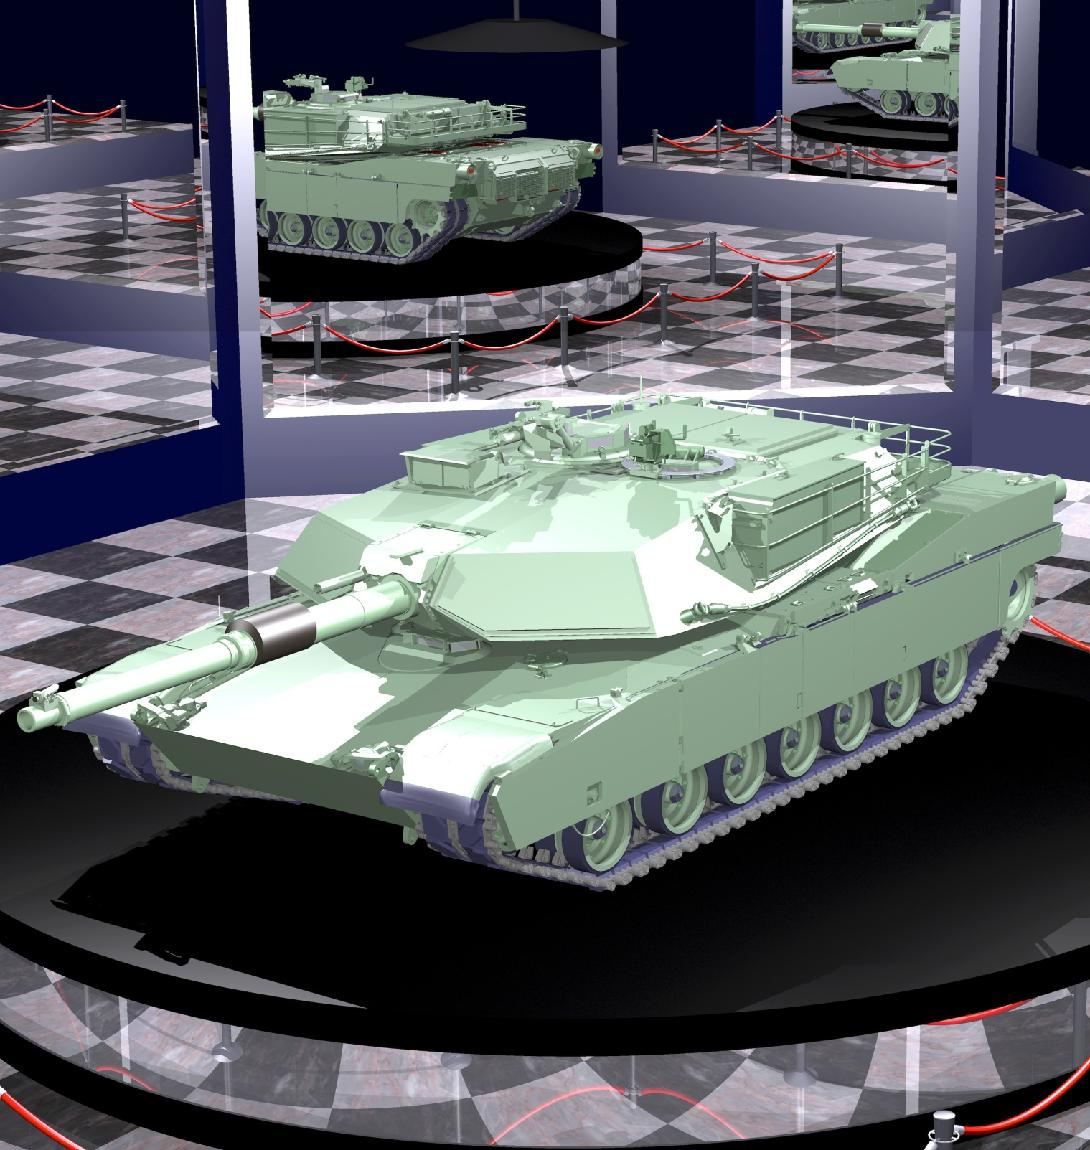
\includegraphics[trim=0.0cm 0.5cm 0.1cm 0.1cm, clip=true, totalheight=0.5\textheight]{Pictures/M1A1.png}
\caption[An M1A1 tank on a pedestal in a mirrored showcase room]{An M1A1 tank on a pedestal in a mirrored showcase room}
\label{M1A1}
\end{figure}  

\subsection{Cell Decomposition}

\hspace{30} Despite   the   wide   applicability   and   attention   received   by   boundary  
representations,   it   gradually   became   exciting   to   research   new   ways   of  
representing   objects   explicitly   by   their   volume   –   a   collection   of   minute   cells   of   a  
partition   of   $\mathbb{E}^3 $.   Some   widely   used   data   structures   under  
this   representational   paradigm   are   hierarchical   in   nature   and   recursively  
decompose   space   until   they   obtain   atomic   blocks   for   which   no   further  
 decomposition   is   necessary.   Although   this   representation   scheme   is   not   widely  
used   within   the   BRL-­CAD   package,   we   thought   it   important   to   highlight   the   prolific  
developments   in   this   area   of   research.   Due   to   the   frequent   use   of   hierarchical  
data   structures   in   representing   images   in   the   domains   of   computer   vision,  
image   processing   and   computer   graphics,   the   atomic   blocks   obtained   from  
recursive decomposition are called \textit{picture elements} or \textbf{\textit{pixels}} for short. 

\hspace{30} The   term   \textit{quadtree}   has   been   used   to   describe   hierarchical   data  
structures   which   are   based   on   the   common   property   of   recursive  
decomposition   and   can   be   differentiated   by   the   type   of   data   being   represented,  
the   principle   guiding   the   decomposition   process   and   the   resolution   of   that  
decomposition   (the   number   of   times   the   decomposition   is   applied   –   whether  
fixed   or   variable).   The   most   common   quadtree   is   the   region   quadtree   due   to  
Klinger   and   Dyer \cite{24}   and   was   coined   by   Hunter \cite{25}.It   is   based   on   the  
successive   subdivision   of   the   image   array   into   four   (4)   equal-­sized   quadrants  
which   may   be   recursively   subdivided   until   pixels   are   obtained.   In   the   tree  
representation,   the   root   node   corresponds   to   the   entire   array,   each   child   of   a  
node   represents   a   quadrant   of   the   region   the   parent   node   represents   while   a  
leaf   node   represents   an   atomic   block   (usually   a   pixel).   A   leaf   node   may   be  
black   or   white   depending   on   whether   its   pixel   is   entirely   inside   or   outside   the  
represented region. It may be gray if it is an internal node of the tree.  

\hspace{30} As   initiated   by   the   aforementioned   research   carried   out   by   Finkel   and  
Bentley \cite{26},   hierarchical   data   structures   can   be   used   to   represent   images   in  
three­dimensional   space   and   even   higher.   The   \textit{\textbf{octree}}   data   structure   is   the  
three­-dimensional   analog   of   the   quadtree.   Here,   an   image   is   first   represented   in  
the   form   of   a   cubical   volume   and   then   recursively   decomposed   into   eight   (8)  
congruent   disjoint   cubes   called   octants   until   cubes   are   obtained   or   a   uniform   or  
predetermined   decomposition   is   reached.   The   original   structure   of   a   quadtree  
encodes   it   as   a   tree   structure   using   pointers.   This   additional   memory   overhead  
posed   a   problem   and   prompted   two   (2)   approaches   to   curbing   it.   Although   it   is  
difficult   to   put   a   finger   on   who   exactly   developed   the   first   approach   to   solving  
this   problem,   it   is   an   efficient   method   which   treats   the   image   as   a   collection   of  
leaf   nodes   each   of   which   is   encoded   by   a   base   4   number   termed   a   \textit{locational  
code}. 

\hspace{30} The   second   approach   to cell decomposition due   to   Kawaguchi   and   Endo \cite{27}   is   termed   a  
$\textit{\textbf{\mathbf{DF}-­expression}}$.   It   represents   the   image   in   the   form   of   a   traversal   of   the   nodes  
of   its   quadtree   –   a   compact   representation   in   which   each   node   type   is   encoded  
with   2   bits.   Although   it   is   not   easy   to   use   when   random   access   to   nodes   is  
required,   it   has   been   shown   to   be   faster   than   the   former   for   a   static   collection   of  
nodes   representing   images   in   higher   dimensional   space   using   an   efficient  
pointer­-based implementation.

\hspace{30} Rectangular   data   is   often   used   to   approximate   objects   in   an   image   for  
which   they   serve   as   the   minimum   rectilinear   enclosing   object.   Indeed,   bounding  
rectangles   are   used   in   cartographic   applications   to   approximate   lakes,   forests,  
hills,   etc.   The   first   representation   of   quadtrees   holding   rectangular   data   was  
due   to   Hinrichs   and   Nievergelt \cite{28}.   In   this   representation,   each   rectangle   is  
seen   as   a   cartesian   product   of   two   line   intervals   each   analogous   to   an   interval  
tree   holding   the   interval's   centroid   and   extent.   The   rectangles   are   reduced   to  
points   in   three­dimensional   space   and   then   the   problem   is   treated   as   if   dealing  
with   a   collection   of   points.   Another   such   representation   is   the   region­-based  
\textit{MX­CIF   quadtree}   in   which   each   rectangle   is   associated   with   the   quadtree   node  
corresponding   to   the   smallest   block   containing   it   entirely.   The   subdivision  
ceases   whenever   a   node's   block   contains   no   rectangles   or   is   smaller   than   a  
predetermined   threshold   size.   Yet   another   such   data   structure   arose   called   the  
\textit{R­-tree}   developed   by   Guttman \cite{29}   in   which   each   node   in   the   R-­tree   is   a  
d - ­dimensional   rectangle   enclosing   its   child   nodes.   Its   leaf   nodes   are   the  
rectangles   in   the   database.   Each   rectangle   may   be   contained   in   several   nodes  
each   of   which   had   to   be   visited   before   ascertaining   the   presence   or   absence   of  
a   particular   rectangle.   This   lead   the   retrieval   of   rectangles   to   be   to   slow; a  
problem   which   was   alleviated   by   the   implementation   of   an   \textit{${R^{+}}$-tree}   in   which  
each   rectangle   is   associated   with   with   several   non­overlapping   bounding  
rectangles.   The   retrieval   time   of   the   R­-tree   is   sped   up   at   the   expense   of   an  
increase in the tree's height.

\hspace{30} We   now   conclude   our   review   of   hierarchical   data   structures   by   looking   at  
data   structures   which   explicitly   specify   the   boundaries   of   regions.   They   are  
called   Polygonal   Maps   ($\mathbf{PM}$) – a   collection   of   polygons   which   can   either   be  
vertex-­based   or   edge-­based.   The   vertex-­based   Polygon   Maps   quadtree   or   $PM_1$
 quadtree   in   two­-dimensions   was   due   to   \cite{30}.   The   \textit{$PM_1$   quadtree}   was   based   on   a  
decomposition   rule   stipulating   that   positioning   occurs   as   long   as   a   block  
contained   more   than   one   line   segment   unless   the   line   segments   are   all   incident  
at   the   same   vertex   in   the   same   block.   The   three-­dimensional   $PM_1$   octree   data  
structure   is   quite   useful   as   it   is   more   forgiving   on   memory   than   the   conventional  
octree   when   representing   objects.   The   edge­-based   variant   of   the   PM   quadtree also dubbed the \textit{PMR quadtree}   uses   a   probabilistic   splitting   rule   in   which   nodes   contain   a  
variable number of line segments.

\hspace{30} Shown   below   in Figure 2.6 is   a   Sphere   Flake   drawn   using   BRL-­CAD   represented  
using   an   octree   with   five   levels   of   recursion,   specular   reflections,   multiple   light  
sources,   environment   mapping,   checkered   texture   synthesis,   ambient  
occlusion, and soft shadows.

\begin{figure}[htbp]
\centering
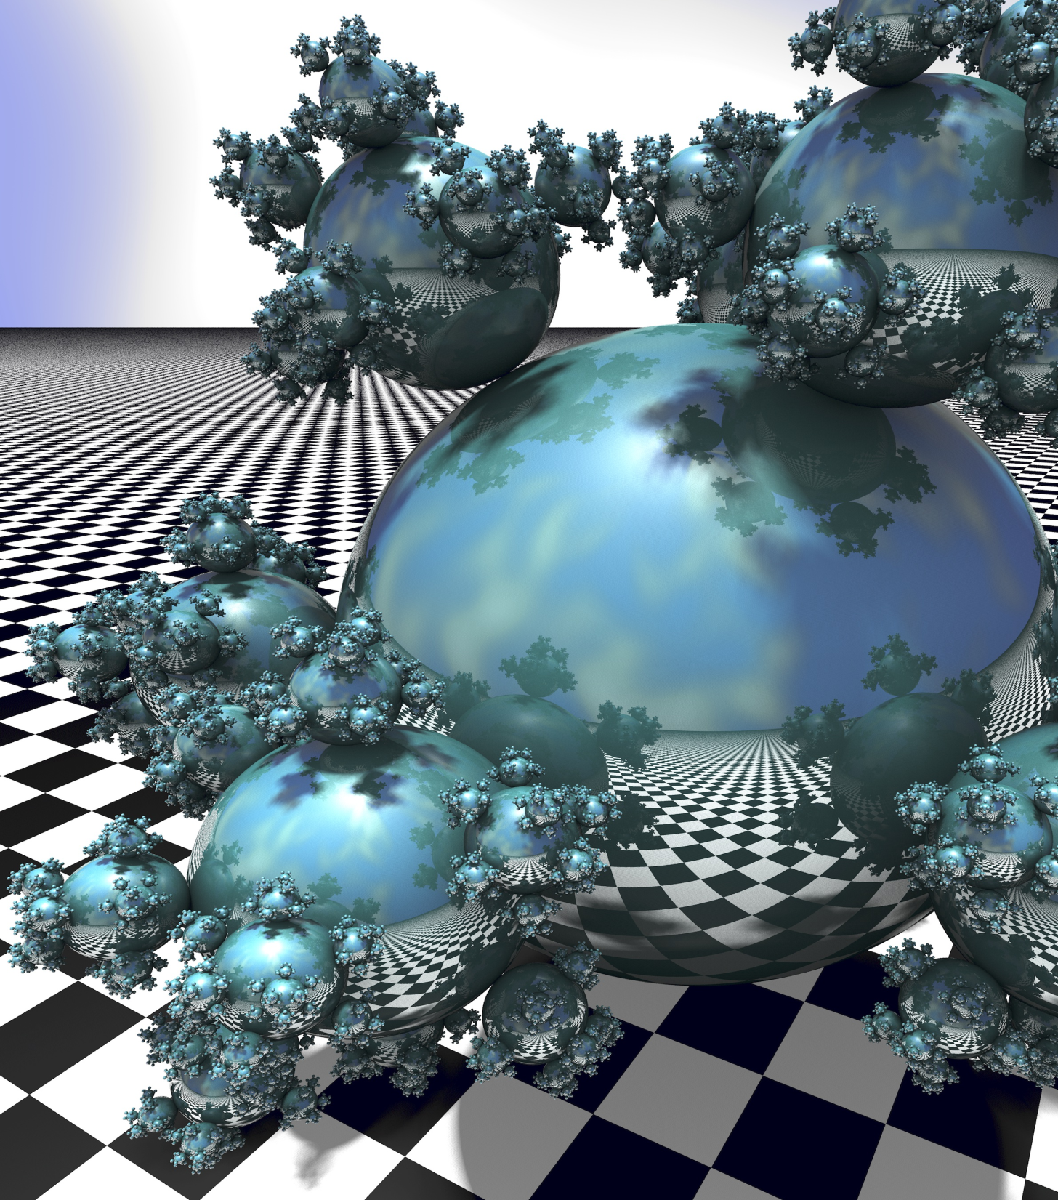
\includegraphics[trim=0.0cm 0.5cm 0.1cm 0.1cm, clip=true, totalheight=0.5\textheight]{Pictures/Sphere.png}
\caption[Model of a Sphere Flake]{Model of a Sphere Flake}
\label{Sphere}
\end{figure}

\clearpage
%------------------------------------------------------------------------------------------------------

%-------------------------------------------------------------------------------------------------------
%		NON - MANIFOLD GEOMETRY
%-------------------------------------------------------------------------------------------------------
\section{Non-manifold Geometry}

\hspace{30} So   far,   we   have   explored   the   modeling   of   manifold   objects – objects   with  
the   property   that   each   of   its   points   have   neighbourhoods   which   are  
homeomorphic   to   $\mathbb{E}^3$.   These   manifolds   can  also   be   seen   as   
r-­sets   which   were   defined   by   Requicha   in   \cite{5}.   Lines   and   circles  are   
one-­dimensional   manifolds   while   primitives   such   as   tori,   spheres,   cones, 
cylinders,heart­-shape,etc are examples of three­-dimensional manifolds.

\hspace{30} We   now   throw   some   light   on   geometric   algorithms   used   to   represent  
non­manifolds   ­   objects   which   have   points   with   neighbourhoods   which   are   not  
homeomorphic   to   $\mathbb{E}^3$ .   While   lines   and   circles   are   one-­dimensional   manifolds,  
figure   eights   are   one­-dimensional   non­-manifolds.   Examples   of   two-­dimensional  
non­-manifolds   may   include   a   cone   touching   another   surface   at   a   single   point,  
faces   meeting   along   a   common   edge,   etc.   Non-­manifolds   usually   arise   when  
topological   structures   such   as   vertices,   edges,   and   faces   hang­off   the   mapped  
boundary   graph   of   an   object.   They   also   naturally   result   from   regularized  
boolean operations in CSG even when input is restricted to manifolds only.  

\begin{figure}[htbp]
\centering
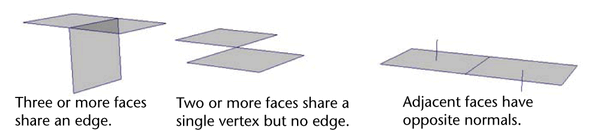
\includegraphics[trim=0.0cm 0.1cm 0.1cm 0.1cm, clip=true, totalheight=0.1\textheight]{Pictures/NMG.png}
\caption[Examples of Non­-Manifold Geometry]{Examples of Non-Manifold Geometry}
\label{NMG}
\end{figure}

\hspace{30} According   to   \cite{2},   non­-manifold   representations   are   representations   which  
allow   volume,   manifold   and   non­-manifold   curves,   surfaces   and   point   elements  
in   a   single   uniform   environment.   Thus,   non-­manifold   modeling   is   seen   as   a  
hybrid   representation   paradigm   which   simultaneously   encompasses   wireframe  
modeling,   surface   modeling   and   solid   modeling.   It   enables   a   smooth   transition  
between   several   representation   schemes   and   the   automatic   detection   of   solid  
enclosures without any need for restructuring or translation.  

\hspace{30} In   \cite{2},   Weiler   developed   the   \textit{radial-­edge}   data   structure   which   can   be  
used   to   represent   non-­manifold   geometry.   NMG   topological   elements   include  
vertices,   edges,   loops,   faces,   shells,   regions   and   models.   The   topological  
information   stored   in   a   non­-manifold   model   consists   of   adjacencies   of  
topological   elements.   An   adjacency   relationship   is   the   adjacency   of   a   group   of  
topological   elements   of   one   type   around   some   other   specific   single   element.

\hspace{30} Thirty­-six   (36)   adjacency   relationships   are   possible   in   non ­manifold   boundary  
representations.   The   radial­-edge   data   structure   employs   \textit{up­pointers}   and  
\textit{down­pointers}   to   depict   the   relative   \textit{“hierarchy”}   which   exists   between   topological  
elements.   The   reader   can   find   more   information   about   data   structures   used   for  
non-­manifold geometric modeling at \cite{31} and \cite{32}. 
 
\hspace{30} In this chapter, we reviewed the work done by researchers in the field of  
geometric modeling which has been applied in the development of the BRL-­CAD viz 
wireframe modeling, surface modeling, solid modeling and non-­manifold modeling.  

\clearpage
%-------------------------------------------------------------------------------------------------------
